\documentclass{beamer}
%\usepackage{beamerthemesplit}
\title{Computational Physics Group Project: \\ Ecosystem: predator and prey}
\author{David Hicks\\ Weiyao Ke \\ Shagun Maheshwari \\ Fan Zhang}
\date{\today}

\begin{document}

\frame{\titlepage}

\section[Outline]{}
\frame{\tableofcontents}

\section{Introduction to eco-system modelling}
\frame
{
  \frametitle{Population interaction of predator and prey in eco-system}
  %Add what you want here
\begin{figure}[htbp]
\begin{center}
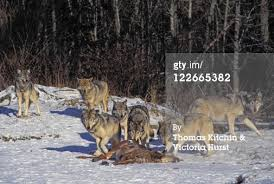
\includegraphics[width=0.9\textwidth]{predator_prey.jpg}
\caption{default}
\label{default}
\end{center}
\end{figure}

  
}
\frame
{
  \frametitle{A simplified determinsitic model L-V equation}
  %Add what you want here
  
}
\frame
{
  \frametitle{Simulation of a eco-system with predator and prey}
  %Add what you want here
  
}

\section{Implementation of the simulation}
\frame
{
  \frametitle{Structural setup}
  %Add what you want here
  
}

\frame
{
  \frametitle{Initialization}
  %Add what you want here
  
}

\frame
{
  \frametitle{time evolution}
  %Add what you want here
  
}

\frame
{
  \frametitle{parameter scanning}
  %Add what you want here
\begin{figure}[htbp]
\begin{center}
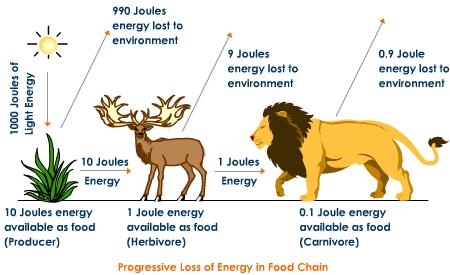
\includegraphics[width=0.9\textwidth]{progressive-energy-loss.jpeg}
\caption{default}
\label{default}
\end{center}
\end{figure}

  
}

\section{Results and discussion}
\frame
{
  \frametitle{results}
  %Add what you want here
  
}


\end{document}
